\chapter{Related Literature and Studies}

This chapter presents the related literature and studies after the thorough search done by the proponents.
This will also present the synthesis of the art, theoretical and conceptual framework to fully understand the research to be done and the definition of terms for a better understanding of the study.

\section*{Reasons why students cheat}

\citeA{nuss1984academic} stated that cheating and competition are not new issues for higher education.
Cheating incidences were observed to be affected by the credit awarded or the weight of the exam \cite{weber1983cheating}.

According to the research 'Undergraduate Student Cheating in Exams' conducted by \citeA{dodeen2012undergraduate}, hard courses, hard courses, hard exams, the desire for good grades, improving one's chances, fear of failure are the reasons why students cheat.

In addition, the article about Reasons Students Plagiarize or Cheat of acdemicintegrity.com stated that students chat because of the belief they will not get caught and that the examination can be aced easily.

The most commonly reported challenge in online assessment is how to maintain academic integrity \cite{hollister2009proctored}, 2009), especially with unproctored assessments \cite{arnold2016cheating}.
\citeA{KERESZTURY20131516} evaluated cheating methods in classic exams which they classified into three categories: information exchange among students, using forbidden materials, and circumventing the assessment process.

\section*{Cheating in Online Examination}

In the research conducted by \citeA{rogers2006faculty} about faculty perceptions about e-cheating during Online testing, Digital cheating is a term used to describe students who find a way to cheat using computer technology.
One specific form of digital cheating is "e-cheating" which specifically relates to the use of the World Wide Web to assist with cheating.

\citeA{rogers2006faculty} also stated the methods of suspected or actual e-cheating by students which are: Email communication, surfing the internet, accessing unauthorized sites, accessing other files/software.

\section*{Online Cheating Prevention}

It is important to make cheating as difficult as possible and to make the punishment of cheating severe \cite{genereux1995circumstances}.
It is also important to take appropriate action against the offender every time a student is caught.
In addition, all students' actions should be reported to a central record-keeping agency to help identify repeated offenders \cite{todd1987cheating}.

\citeA{moten2013examining} explained that students enrolled in distance learning work independently with relative autonomy and anonymity, and instructors may be uncertain who is taking exams or how best to validate student learning.
\citeA{gao2012online} summed the commonly used methods to prevent students from taking online exams from e-cheating are: Setting up time limitations, Exams consist of randomly selected questions from a vast question pool so that each student will have a different exam/test, Comparing the IP addresses to see if two students are in the vicinity of each other, and Using biometrics to reduce the possibility of E-cheating and to authenticate remote students.

Before the above preventions, the adaptation of Online proctoring services is highly recommended to aid academic dishonesty.

\section*{Online Proctoring}

Many institutions have adopted Automated Online Proctoring Technology to promote academic integrity in their online learning environment.
The automated online proctoring is a relatively new technology that uses the student's webcam and microphone to verify and create a secure testing environment that imitates in-person proctoring to prevent cheating \cite{karim2014cheating}.
In addition, automated online proctoring is cost-efficient \cite{atoum2017automated}.

\section*{Distance learning cheating in the Philippines}

Briones of the Department of Education (DepEd) noted that "Distance cheating has always been a challenge even before COVID,".
As the implementation and massive promotion of distance learning began due to COVID19 Pandemic, DepEd appealed to parents and other significant adults to be part of the solution to avoid the possibility of distance cheating as the use of the internet for research and academic purposes has given birth to a big threat in every school or university's academic integrity, as some student resort to or unintentionally commit plagiarism \cite{quieta2020plagiarism}.

Most of the universities adopt remote and proctored examinations. As for academic facilities to be successful and credible in the future, proctoring will be important for students in the verification of their identities and to provide evidence that they are responsible for the achievement of their learning outcomes \cite{dela2015massive}.

\section{Related Studies}

One large-scale study of cheating in online courses and work tasks found that between 26\% and 34\% of students cheated by looking up answers online, as did 20\% of contract employees \cite{corrigan2015deterring}.
Online collusion during asynchronous unproctored exams was detected among engineering students (de Sande, 2015), and over 1,230 massive open online courses, students copied answers during asynchronous unproctored certificates exams using multiple online accounts \cite{northcutt2016detecting}.

The studies above are the same as the present study as they will identify the different cheating behaviors of the students during an unproctored online examination.
But the main focus of the present study is only on the behaviors of students in AMA Computer College Parañaque.

In the research addressing student validation based on face recognition for online learning \cite{labayen2014smowl}, it is stated that without certainty of the authenticity of the online learner's identity, the aspiration towards fully online education is stymied and the evaluation of the knowledge and skills obtained by the online learner is unreliable.

This research is similar to the present study as it will portray the relevance of the validity of students' identity in taking an online examination.
\citeA{frankl2011secure} gave "Secure Exam Environment" (SEE) implemented at the Alpen-Adria-Universität Klagenfurt (AAUK) to be held on student portable pcs without access to local files and resources, for example, the Internet.
The AAUK is using the e-learning-platform "Moodle" (see http://moodle.com) as a teaching and testing tool.
Therefore, the usage of the SEE is embedded in Moodle.

This study has the same objective as the present study. However, the present study also includes face recognition to assure the validity of the test takers.
Also, the present study will not be embedded in the e-learning platform used by AMA Computer College Parañaque, it will be an independent web application that is only intended for the online examination of students.

\section{Local Studies}

An open-ended questionnaire was distributed to 52 students of the University of the Philippines Open University enrolled in a Computer Ethics course at the graduate level where the course, including the final exam, is fully online \cite{ravasco2012technology}.
The first question asked was where students cheat more frequently, and 21 out of 52 which is 40.38\% of the class are convinced that there is more cheating or more possibility of it happening in an online classroom.
One reason a student has stated was: "I believe cheating is more frequent in an online distance course because the information is readily available and accessible.
Once a student goes online, hundreds and hundreds of answers for assignments, quizzes, or tests can be acquired.

The students then asked to offer ways online cheating could be done or is already being done based on their readings, their experiences, and from their observation.
73\% (38/52) mentioned identity impersonation, substitution, or proxy attendance as the most common and perhaps the easiest to get away with.
Here an online student gets another to do the academic work required for him or her.
69\% (36/52) named the search engine and plagiarism duo as a very common way of cheating.
Students would "google" terms, ideas, concepts, and copy-paste their desired portions of their work.
69\% (36/52) referred to unauthorized intellectual networking as another method of cheating.

Students would collaborate dishonestly and even share files in the process.
This involves discussing answers with each other using forums or even personal chat rooms.
The research also let the students provide recommendations regarding preventing online cheating.
62\% of the students (32/52) cited an improvement to the Design of Assessment of the examination environment.
The variety of Test design versions, randomization of items in the question pool, password protection and limit of access to the online test, assessment deployment in a secure web browser (response lockdown) with a "one question per screen" technique.
On the other hand, Monitoring and evaluating of examinations was recommended by 35\% of the students (18/52), Such as Online proctoring using screen viewers or screen capture (ex. join me) and using web cameras could ensure proper monitoring of students in their assessment.

The above study is comparable to the present study about the enumeration of the cheating tendencies of the students and its prevention through automated online proctoring.

\section{Technical Background}

The proposed system is a web-based application to enable broad availability for its end-users.
The process of detecting and recognizing users' faces is handled solely in the browser to provide real-time detection during exams.
Running real-time facial detection can be resource intensive.
To achieve a smoother experience for end-users, the proposed system uses a neural network model optimized for resource-limited devices.
The application will be implemented as a Single-Page Application (SPA).
SPAs are a more dynamic and modern type of web application than standard websites.
User interaction is much more seamless as all data on the page dynamically changes without requesting a new page.

The frontend of Proctor Vue is written using Vue.js, a popular JavaScript framework for creating Single-Page Applications.

The server-side logic is written using ExpressJS, a Node.js web application framework.
The Express application handles requests from the client through the system's Application Programming Interface (API) and retrieves data directly from the database.

The system is deployed through the Amazon Web Services (AWS) ecosystem.
The ExpressJS backend is running on provisioned virtual instances of Amazon Elastic Compute Cloud (EC2).
EC2 instances are essentially virtual computers that live in the cloud, allowing them to be scaled easily as the application's load increases/decreases.
The Vue.js SPA is stored using Amazon Simple Storage Service (S3) and is served using Amazon CloudFront, a content delivery network (CDN).
Serving static content, such as a Single-Page Application, through a CDN provides a faster and more cost-efficient way to deliver the application to users.


\section{Synthesis}

The cited related literature and studies, both foreign and local have some relationship and relevance to the proposed study particularly the concerns on the academic malpractices during the online examination and the need to aid against it using the online proctoring application.

The different studies helped the proponents to gain knowledge and support its ideas for the design and development of the proposed study.
Thus, the potential of the proposed Web-based Automated online proctoring to eliminate cheating activities and creating a fair online assessment has been identified.

\section{Conceptual Framework}

The conceptual framework is the scheme formulated from the related studies that will guide the proponents in the study.

\pagebreak

\begin{figure}[h!]
   \begin{center}
      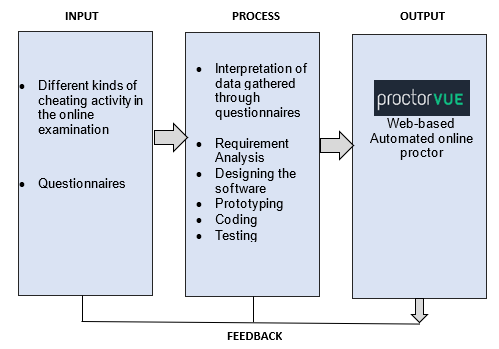
\includegraphics[scale=1.0]{conceptual-framework}
      \caption{Conceptual Paradigm of the Study}
   \end{center}
\end{figure}

\textbf{The Input} consists of the cheating activities encountered in the online examination of AMA Computer College Parañaque and the additional information from the data gathered in the questionnaires.

\textbf{The Process} shows the interpretation and analysis of the gathered data from the questionnaires, analyzing the requirements needed to create the program, designing the software, prototyping, coding both front and backend, and testing.

\textbf{The Output} of the study, Proctor Vue: A web-based automated online proctoring.

